% Sección 7: resultados y análisis (Rol 3, P2). Insertar con % Sección 7: resultados y análisis (Rol 3, P2). Insertar con % Sección 7: resultados y análisis (Rol 3, P2). Insertar con % Sección 7: resultados y análisis (Rol 3, P2). Insertar con \input{seccion_7_resultados}.
% Requiere booktabs y graphicx. Figuras 15-18: scripts/06_analisis_errores.py.
% Cifras: data/processed/lineales_*.csv, no_lineales_*.csv y errores_*.csv.
\section{Resultados y análisis}
\label{sec:resultados}
Se comparan cuatro modelos sobre las mismas filas: persistencia, Ridge sin calendario (el lineal elegido en la sección~5) y los representantes con calendario de Random Forest y HistGB. Las diferencias de MAE se acompañan de intervalos de confianza del 95~\% obtenidos por bootstrap de bloques móviles de 24 filas consecutivas (2000 réplicas), que conserva la autocorrelación de los errores; los bloques se forman sobre filas, por lo que un hueco de medición puede quedar dentro de un bloque.

\subsection{Comparación global}
\label{sec:comparacion}
La Tabla~\ref{tab:resultados} y la Fig.~\ref{fig:comparacion} resumen el desempeño. En validación, Random Forest obtiene el menor MAE (2,985) y mejora un 11,6~\% sobre la persistencia, frente al 9,5~\% de HistGB y el 7,0~\% de Ridge. En prueba, los dos modelos de árboles quedan prácticamente empatados en MAE (2,413 y 2,428, mejoras de 14,7~\% y 14,2~\%) y HistGB logra el menor RMSE (4,347). Los intervalos de la diferencia con la persistencia excluyen el cero para los tres modelos en ambos bloques. Frente a Ridge, Random Forest reduce el MAE en 0,16 µg/m³ en validación (IC $[-0{,}22;\,-0{,}10]$) y 0,21 en prueba ($[-0{,}28;\,-0{,}15]$); HistGB, en 0,08 ($[-0{,}15;\,-0{,}02]$) y 0,20 ($[-0{,}27;\,-0{,}12]$). La ganancia de los árboles es, por tanto, consistente pero modesta en términos absolutos: del orden de 0,2--0,4 µg/m³ por hora.

\begin{table}[t]
\centering
\caption{Desempeño en validación y prueba. Mejora: reducción porcentual del MAE frente a la persistencia en el mismo bloque. $\Delta$: diferencia de MAE frente a persistencia (µg/m³) con IC 95~\% por bootstrap de bloques.}
\label{tab:resultados}
\small
\setlength{\tabcolsep}{3.5pt}
\begin{tabular}{@{}lrrrrl@{}}
\toprule
Modelo & MAE & RMSE & $R^2$ & Mejora & $\Delta$ [IC 95~\%] \\
\midrule
\multicolumn{6}{@{}l}{\emph{Validación (jul--dic 2023, $n=4024$)}} \\
Persistencia & 3,378 & 5,143 & 0,700 & -- & -- \\
Ridge & 3,141 & 4,755 & 0,744 & 7,0~\% & $-0{,}24$ [$-0{,}29$; $-0{,}18$] \\
Random Forest & \textbf{2,985} & \textbf{4,565} & \textbf{0,764} & 11,6~\% & $-0{,}39$ [$-0{,}47$; $-0{,}32$] \\
HistGB & 3,057 & 4,617 & 0,758 & 9,5~\% & $-0{,}32$ [$-0{,}41$; $-0{,}24$] \\
\midrule
\multicolumn{6}{@{}l}{\emph{Prueba (ene--abr 2024, $n=2701$)}} \\
Persistencia & 2,829 & 5,265 & 0,631 & -- & -- \\
Ridge & 2,626 & 4,766 & 0,698 & 7,2~\% & $-0{,}20$ [$-0{,}27$; $-0{,}13$] \\
Random Forest & \textbf{2,413} & 4,486 & 0,732 & 14,7~\% & $-0{,}42$ [$-0{,}51$; $-0{,}31$] \\
HistGB & 2,428 & \textbf{4,347} & \textbf{0,749} & 14,2~\% & $-0{,}40$ [$-0{,}52$; $-0{,}28$] \\
\bottomrule
\end{tabular}
\end{table}

\begin{figure*}[t]
\centering
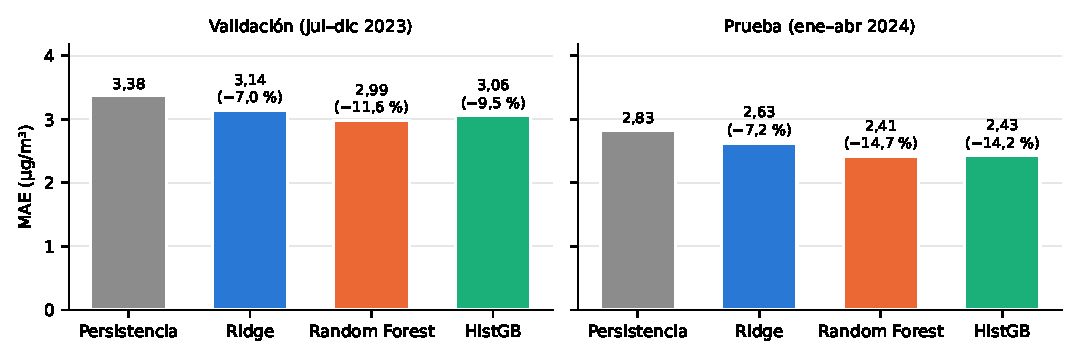
\includegraphics[width=\textwidth]{figures/15_comparacion_modelos.pdf}
\caption{MAE por modelo y bloque. Entre paréntesis, la reducción del MAE frente a la persistencia en el mismo bloque.}
\label{fig:comparacion}
\end{figure*}

El MAE de prueba es menor que el de validación para todos los modelos, incluida la persistencia, y el $R^2$ también es menor. Ambos hechos se explican por el cambio de distribución descrito en la sección~3: enero--abril de 2024 tiene concentraciones más bajas y menos variables, de modo que los errores absolutos se reducen sin que el problema sea más fácil en términos relativos. Por la misma razón, el MAE de la validación cruzada interna (4,82 para Random Forest) es mayor: su primera ventana, en el invierno de 2022, tiene un MAE de 6,68, frente a 3,42 en la tercera.

\subsection{Aporte del calendario}
\label{sec:calendario}
La Tabla~\ref{tab:calendario} compara cada familia con y sin calendario en validación, con la misma búsqueda de hiperparámetros. En los modelos lineales el calendario empeora el MAE alrededor de un 2~\%, con un intervalo que excluye el cero; en los de árboles lo mejora un 3,2~\% (Random Forest) y un 2,4~\% (HistGB), también con intervalos que excluyen el cero. La importancia por permutación (Fig.~\ref{fig:importancia}) localiza el aporte en la hora pronosticada: permutarla aumenta el MAE de validación en 0,36 µg/m³ en Random Forest y 0,49 en HistGB, mientras que permutar el día de la semana no lo cambia. Una interpretación coherente es que el efecto de la hora no es aditivo: las mayores ganancias de los árboles sobre Ridge se concentran entre las 17 y las 21~h (sección~\ref{sec:errores}), cuando la concentración cambia de tendencia a diario, y esa interacción entre hora y nivel reciente no puede representarse con un seno y un coseno sumados linealmente.

\begin{table}[t]
\centering
\caption{MAE de validación sin y con calendario. $\Delta$: con menos sin (µg/m³), IC 95~\% por bootstrap de bloques.}
\label{tab:calendario}
\small
\setlength{\tabcolsep}{3pt}
\begin{tabular}{@{}lrrrl@{}}
\toprule
Familia & Sin & Con & Cambio & $\Delta$ [IC 95~\%] \\
\midrule
Ridge & 3,141 & 3,205 & $+2{,}0$~\% & $0{,}06$ [$0{,}02$; $0{,}11$] \\
Lasso & 3,142 & 3,205 & $+2{,}0$~\% & $0{,}06$ [$0{,}02$; $0{,}11$] \\
Random Forest & 3,083 & 2,985 & $-3{,}2$~\% & $-0{,}10$ [$-0{,}13$; $-0{,}06$] \\
HistGB & 3,132 & 3,057 & $-2{,}4$~\% & $-0{,}07$ [$-0{,}12$; $-0{,}02$] \\
\bottomrule
\end{tabular}
\end{table}

\subsection{Importancia de variables}
\label{sec:importancia}
La importancia se mide como el aumento del MAE de validación al permutar una variable, con 20 repeticiones (Fig.~\ref{fig:importancia}); para la hora y el día se permuta la variable original, de modo que su seno y coseno, o sus indicadores, se alteran juntos. En ambos modelos domina la medición actual: permutarla eleva el MAE en 6,76 (Random Forest) y 6,97 µg/m³ (HistGB). Le siguen la hora (0,36 y 0,49) y el rezago de una hora (0,28 y 0,33); el resto aporta menos de 0,15. Este patrón coincide con la autocorrelación parcial de la sección~3, en la que la dependencia se concentra en los primeros rezagos.

\begin{figure}[t]
\centering
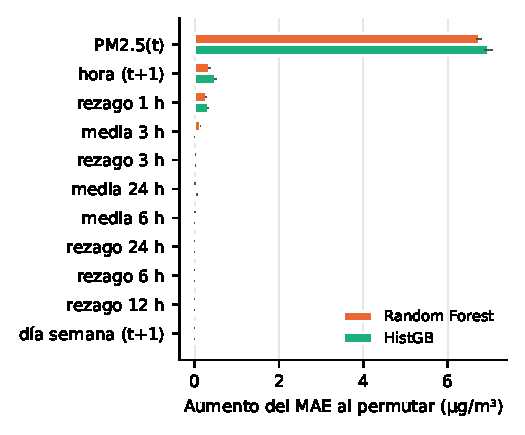
\includegraphics[width=\columnwidth]{figures/16_importancia_variables.pdf}
\caption{Importancia por permutación en validación: aumento del MAE al permutar cada variable (media y desviación de 20 repeticiones).}
\label{fig:importancia}
\end{figure}

Estas cifras tienen tres limitaciones. Primero, las variables de historial están muy correlacionadas: permutar una sola crea combinaciones de entrada que no ocurren en los datos y, a la vez, sus sustitutas pueden compensar su ausencia. Una importancia baja de, por ejemplo, la media de 6~h no implica que la variable sea irrelevante, sino que su información ya está en otras. La distorsión es visible en HistGB, donde permutar conjuntamente las nueve variables de historial aumenta el MAE menos (6,49) que permutar solo la medición actual (6,97). Segundo, la importancia por impureza de Random Forest, calculada en entrenamiento, ordena las variables de forma distinta (medición actual 0,65, media de 3~h 0,21 y rezago de 1~h 0,08) porque reparte el mérito entre variables correlacionadas y favorece las continuas; por eso se reporta solo como contraste. Tercero, ninguna de estas medidas es causal: describen de qué depende el modelo, no qué determina la concentración.

\subsection{Análisis de errores por hora y por mes}
\label{sec:errores}
La Fig.~\ref{fig:hora-mes} desagrega el MAE. Por hora, todos los modelos fallan más entre las 12 y las 15~h de validación, con MAE de 3,7 a 4,8 µg/m³, cuando la concentración sube y cambia con rapidez. La persistencia, que repite el último valor, sufre además en las transiciones: alcanza 5,07 a las 17~h y 3,35 a la 1~h. Allí los árboles obtienen sus mayores ganancias: a las 17~h Random Forest baja a 3,66 frente a 3,95 de Ridge, y a las 19~h, a 2,28 frente a 2,98. En la madrugada y la mañana (3 a 9~h) los cuatro modelos se comportan de forma muy parecida, y entre las 4 y las 7~h la persistencia es incluso ligeramente mejor, lo que indica que en ese tramo la serie cambia poco y la información adicional no aporta.

Por mes, el error es mayor entre septiembre y octubre de 2023 (MAE de 3,2 a 3,6 en todos los modelos) y mínimo en febrero de 2024 (1,9 a 2,1), y vuelve a subir en marzo y abril de 2024. Las diferencias entre meses son mayores que las diferencias entre modelos, por lo que el periodo evaluado condiciona la cifra global tanto como el modelo elegido. El orden de los modelos se mantiene casi todos los meses: la persistencia es la peor en los diez meses, y Random Forest supera a Ridge en nueve, con septiembre de 2023 como excepción.

\begin{figure*}[t]
\centering
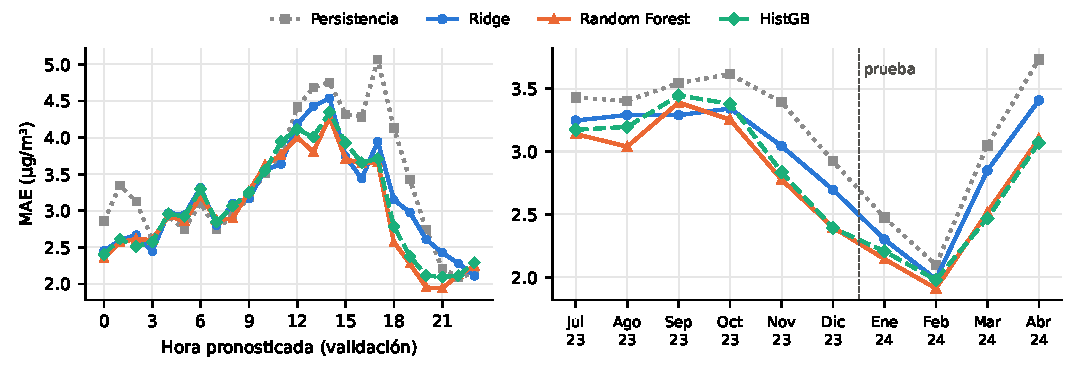
\includegraphics[width=\textwidth]{figures/17_errores_hora_mes.pdf}
\caption{MAE por hora pronosticada en validación (izquierda) y por mes en validación y prueba (derecha). La línea discontinua separa ambos bloques.}
\label{fig:hora-mes}
\end{figure*}

\subsection{Régimen de concentraciones altas}
\label{sec:regimen-alto}
La Fig.~\ref{fig:nivel} agrupa las horas según la concentración observada, usando como cortes la guía diaria de la OMS y sus metas intermedias~\cite{who_aqg_2021}; 50 µg/m³ coincide además con el ECA peruano~\cite{minam_eca_2017}. Esos valores se definen sobre promedios de 24~h y aquí solo sirven para agrupar horas. El MAE crece con la concentración en todos los modelos, y por encima de 50 µg/m³ el sesgo es claramente negativo: los modelos subestiman los episodios. Parte de ese sesgo es mecánica, porque agrupar por el valor observado selecciona las horas en que la concentración subió por encima de lo esperable con la información disponible, y cualquier predictor regresa hacia la media en ellas. Aun así, describe lo que ocurriría en un episodio real.

\begin{figure*}[t]
\centering
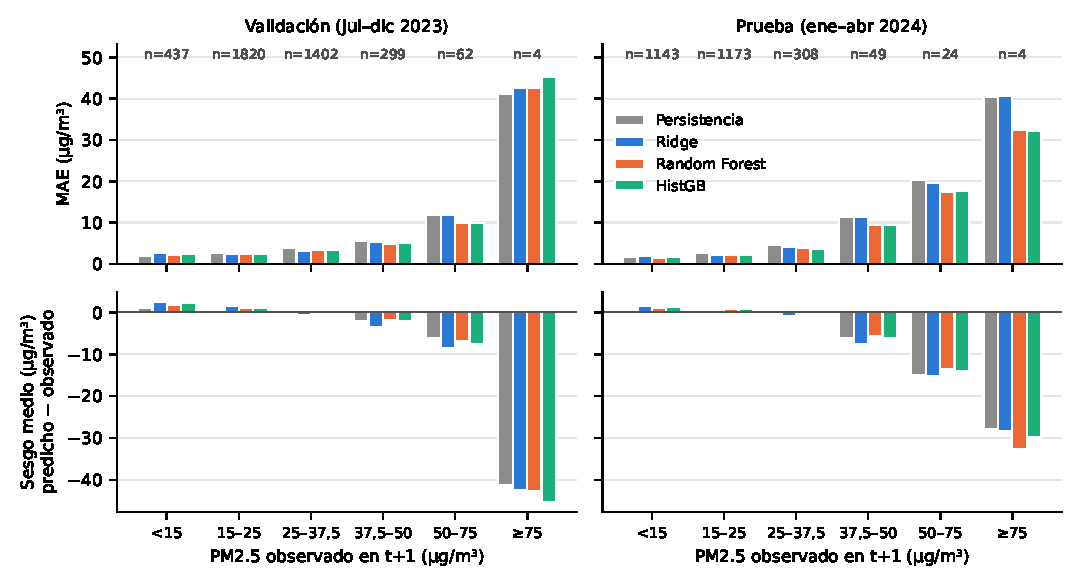
\includegraphics[width=\textwidth]{figures/18_errores_por_nivel.pdf}
\caption{MAE (arriba) y sesgo medio, predicho menos observado (abajo), por nivel de PM2.5 observado en $t+1$. Se indica el número de horas de cada nivel; el último tramo tiene solo cuatro horas por bloque.}
\label{fig:nivel}
\end{figure*}

La Tabla~\ref{tab:regimen} evalúa dos definiciones del régimen alto. La primera es un umbral fijo de 59,25 µg/m³, el percentil 90 de la respuesta en entrenamiento; por el descenso de las concentraciones solo lo superan 16 horas de validación y 17 de prueba. La segunda es el decil superior de cada bloque (desde 36,8 µg/m³ en validación y 27,5 en prueba), con muestra suficiente para comparar. En el decil superior el MAE es entre dos y cuatro veces el del resto de horas (por ejemplo, 5,89 frente a 2,66 para Random Forest en validación y 6,80 frente a 1,92 en prueba). Random Forest y HistGB mejoran a la persistencia en ese decil entre un 8,7~\% y un 18,3~\%, con intervalos que excluyen el cero en ambos bloques, mientras que la mejora de Ridge es pequeña (1,7~\% y 5,3~\%) y en validación no se distingue de cero. Con el umbral fijo, en prueba los árboles reducen el MAE en unos 5,5 µg/m³ frente a la persistencia (IC $[-7{,}8;\,-2{,}5]$ para Random Forest), pero su sesgo sigue cerca de $-22{,}5$ µg/m³; en validación ninguna diferencia es concluyente. Con tan pocas horas, estas cifras son indicativas.

\begin{table}[t]
\centering
\caption{Régimen alto. Umbral fijo: respuesta $\geq 59{,}25$ µg/m³ (p90 de entrenamiento). Decil: 10~\% superior de cada bloque. Mejora frente a persistencia; * indica que el IC 95~\% de la diferencia de MAE excluye el cero.}
\label{tab:regimen}
\small
\setlength{\tabcolsep}{3pt}
\begin{tabular}{@{}lrrrrrr@{}}
\toprule
& \multicolumn{2}{c}{Decil, val.} & \multicolumn{2}{c}{Decil, prueba} & \multicolumn{2}{c}{Umbral, prueba} \\
\cmidrule(lr){2-3}\cmidrule(lr){4-5}\cmidrule(l){6-7}
Modelo & MAE & Mejora & MAE & Mejora & MAE & Mejora \\
\midrule
$n$ & \multicolumn{2}{c}{403} & \multicolumn{2}{c}{272} & \multicolumn{2}{c}{17} \\
Persistencia & 6,74 & -- & 8,08 & -- & 29,05 & -- \\
Ridge & 6,63 & 1,7~\% & 7,65 & 5,3~\%* & 28,28 & 2,6~\% \\
Random Forest & 5,89 & 12,6~\%* & 6,80 & 15,9~\%* & 23,50 & 19,1~\%* \\
HistGB & 6,15 & 8,7~\%* & 6,59 & 18,3~\%* & 23,44 & 19,3~\%* \\
\bottomrule
\end{tabular}
\end{table}

La subestimación persistente es coherente con la limitación señalada en la sección~\ref{sec:no-lineales}: los árboles promedian valores observados en hojas grandes y no pueden anticipar un pico que la historia reciente no anuncia. Sin variables meteorológicas ni de emisiones, el historial de la propia serie no contiene la información necesaria para prever el inicio de un episodio.

\subsection{Respuesta a las preguntas de investigación}
\label{sec:respuestas}
\textbf{P1.} Los modelos de árboles mejoran a la persistencia entre un 9,5~\% y un 11,6~\% en MAE en validación y alrededor de un 14~\% en prueba (unos 0,4 µg/m³ por hora), frente al 7~\% de Ridge. La mejora es estadísticamente consistente, pero pequeña en términos absolutos: la persistencia sigue siendo una referencia exigente a una hora.

\textbf{P2.} El calendario aporta solo en los modelos que pueden combinarlo con el historial. En los de árboles reduce el MAE de validación un 2--3~\%, y el aporte proviene de la hora pronosticada; el día de la semana no aporta en ningún modelo. En los lineales, el calendario empeora ligeramente el MAE.

\textbf{P3.} Sí. En el decil superior el MAE es entre dos y cuatro veces el del resto, y por encima de 50 µg/m³ todos los modelos subestiman de forma sistemática. Los árboles conservan, e incluso amplían, su ventaja relativa sobre la persistencia en ese régimen; la de Ridge se reduce a un 2--5~\% y en validación no se distingue de cero. Ningún modelo resuelve la subestimación de los picos, que es la principal limitación para un uso sanitario del pronóstico.
.
% Requiere booktabs y graphicx. Figuras 15-18: scripts/06_analisis_errores.py.
% Cifras: data/processed/lineales_*.csv, no_lineales_*.csv y errores_*.csv.
\section{Resultados y análisis}
\label{sec:resultados}
Se comparan cuatro modelos sobre las mismas filas: persistencia, Ridge sin calendario (el lineal elegido en la sección~5) y los representantes con calendario de Random Forest y HistGB. Las diferencias de MAE se acompañan de intervalos de confianza del 95~\% obtenidos por bootstrap de bloques móviles de 24 filas consecutivas (2000 réplicas), que conserva la autocorrelación de los errores; los bloques se forman sobre filas, por lo que un hueco de medición puede quedar dentro de un bloque.

\subsection{Comparación global}
\label{sec:comparacion}
La Tabla~\ref{tab:resultados} y la Fig.~\ref{fig:comparacion} resumen el desempeño. En validación, Random Forest obtiene el menor MAE (2,985) y mejora un 11,6~\% sobre la persistencia, frente al 9,5~\% de HistGB y el 7,0~\% de Ridge. En prueba, los dos modelos de árboles quedan prácticamente empatados en MAE (2,413 y 2,428, mejoras de 14,7~\% y 14,2~\%) y HistGB logra el menor RMSE (4,347). Los intervalos de la diferencia con la persistencia excluyen el cero para los tres modelos en ambos bloques. Frente a Ridge, Random Forest reduce el MAE en 0,16 µg/m³ en validación (IC $[-0{,}22;\,-0{,}10]$) y 0,21 en prueba ($[-0{,}28;\,-0{,}15]$); HistGB, en 0,08 ($[-0{,}15;\,-0{,}02]$) y 0,20 ($[-0{,}27;\,-0{,}12]$). La ganancia de los árboles es, por tanto, consistente pero modesta en términos absolutos: del orden de 0,2--0,4 µg/m³ por hora.

\begin{table}[t]
\centering
\caption{Desempeño en validación y prueba. Mejora: reducción porcentual del MAE frente a la persistencia en el mismo bloque. $\Delta$: diferencia de MAE frente a persistencia (µg/m³) con IC 95~\% por bootstrap de bloques.}
\label{tab:resultados}
\small
\setlength{\tabcolsep}{3.5pt}
\begin{tabular}{@{}lrrrrl@{}}
\toprule
Modelo & MAE & RMSE & $R^2$ & Mejora & $\Delta$ [IC 95~\%] \\
\midrule
\multicolumn{6}{@{}l}{\emph{Validación (jul--dic 2023, $n=4024$)}} \\
Persistencia & 3,378 & 5,143 & 0,700 & -- & -- \\
Ridge & 3,141 & 4,755 & 0,744 & 7,0~\% & $-0{,}24$ [$-0{,}29$; $-0{,}18$] \\
Random Forest & \textbf{2,985} & \textbf{4,565} & \textbf{0,764} & 11,6~\% & $-0{,}39$ [$-0{,}47$; $-0{,}32$] \\
HistGB & 3,057 & 4,617 & 0,758 & 9,5~\% & $-0{,}32$ [$-0{,}41$; $-0{,}24$] \\
\midrule
\multicolumn{6}{@{}l}{\emph{Prueba (ene--abr 2024, $n=2701$)}} \\
Persistencia & 2,829 & 5,265 & 0,631 & -- & -- \\
Ridge & 2,626 & 4,766 & 0,698 & 7,2~\% & $-0{,}20$ [$-0{,}27$; $-0{,}13$] \\
Random Forest & \textbf{2,413} & 4,486 & 0,732 & 14,7~\% & $-0{,}42$ [$-0{,}51$; $-0{,}31$] \\
HistGB & 2,428 & \textbf{4,347} & \textbf{0,749} & 14,2~\% & $-0{,}40$ [$-0{,}52$; $-0{,}28$] \\
\bottomrule
\end{tabular}
\end{table}

\begin{figure*}[t]
\centering
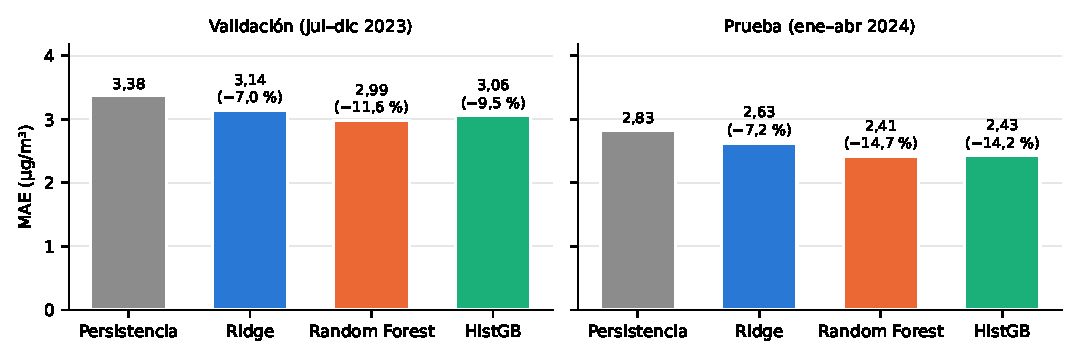
\includegraphics[width=\textwidth]{figures/15_comparacion_modelos.pdf}
\caption{MAE por modelo y bloque. Entre paréntesis, la reducción del MAE frente a la persistencia en el mismo bloque.}
\label{fig:comparacion}
\end{figure*}

El MAE de prueba es menor que el de validación para todos los modelos, incluida la persistencia, y el $R^2$ también es menor. Ambos hechos se explican por el cambio de distribución descrito en la sección~3: enero--abril de 2024 tiene concentraciones más bajas y menos variables, de modo que los errores absolutos se reducen sin que el problema sea más fácil en términos relativos. Por la misma razón, el MAE de la validación cruzada interna (4,82 para Random Forest) es mayor: su primera ventana, en el invierno de 2022, tiene un MAE de 6,68, frente a 3,42 en la tercera.

\subsection{Aporte del calendario}
\label{sec:calendario}
La Tabla~\ref{tab:calendario} compara cada familia con y sin calendario en validación, con la misma búsqueda de hiperparámetros. En los modelos lineales el calendario empeora el MAE alrededor de un 2~\%, con un intervalo que excluye el cero; en los de árboles lo mejora un 3,2~\% (Random Forest) y un 2,4~\% (HistGB), también con intervalos que excluyen el cero. La importancia por permutación (Fig.~\ref{fig:importancia}) localiza el aporte en la hora pronosticada: permutarla aumenta el MAE de validación en 0,36 µg/m³ en Random Forest y 0,49 en HistGB, mientras que permutar el día de la semana no lo cambia. Una interpretación coherente es que el efecto de la hora no es aditivo: las mayores ganancias de los árboles sobre Ridge se concentran entre las 17 y las 21~h (sección~\ref{sec:errores}), cuando la concentración cambia de tendencia a diario, y esa interacción entre hora y nivel reciente no puede representarse con un seno y un coseno sumados linealmente.

\begin{table}[t]
\centering
\caption{MAE de validación sin y con calendario. $\Delta$: con menos sin (µg/m³), IC 95~\% por bootstrap de bloques.}
\label{tab:calendario}
\small
\setlength{\tabcolsep}{3pt}
\begin{tabular}{@{}lrrrl@{}}
\toprule
Familia & Sin & Con & Cambio & $\Delta$ [IC 95~\%] \\
\midrule
Ridge & 3,141 & 3,205 & $+2{,}0$~\% & $0{,}06$ [$0{,}02$; $0{,}11$] \\
Lasso & 3,142 & 3,205 & $+2{,}0$~\% & $0{,}06$ [$0{,}02$; $0{,}11$] \\
Random Forest & 3,083 & 2,985 & $-3{,}2$~\% & $-0{,}10$ [$-0{,}13$; $-0{,}06$] \\
HistGB & 3,132 & 3,057 & $-2{,}4$~\% & $-0{,}07$ [$-0{,}12$; $-0{,}02$] \\
\bottomrule
\end{tabular}
\end{table}

\subsection{Importancia de variables}
\label{sec:importancia}
La importancia se mide como el aumento del MAE de validación al permutar una variable, con 20 repeticiones (Fig.~\ref{fig:importancia}); para la hora y el día se permuta la variable original, de modo que su seno y coseno, o sus indicadores, se alteran juntos. En ambos modelos domina la medición actual: permutarla eleva el MAE en 6,76 (Random Forest) y 6,97 µg/m³ (HistGB). Le siguen la hora (0,36 y 0,49) y el rezago de una hora (0,28 y 0,33); el resto aporta menos de 0,15. Este patrón coincide con la autocorrelación parcial de la sección~3, en la que la dependencia se concentra en los primeros rezagos.

\begin{figure}[t]
\centering
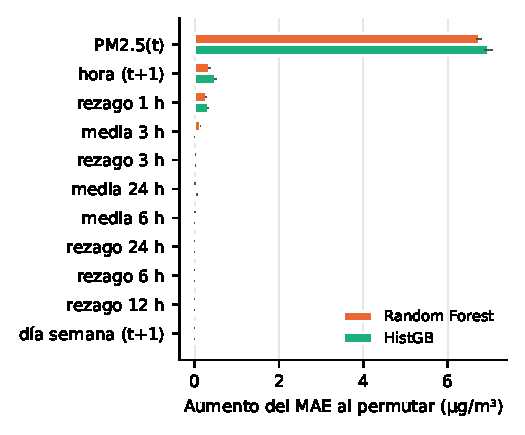
\includegraphics[width=\columnwidth]{figures/16_importancia_variables.pdf}
\caption{Importancia por permutación en validación: aumento del MAE al permutar cada variable (media y desviación de 20 repeticiones).}
\label{fig:importancia}
\end{figure}

Estas cifras tienen tres limitaciones. Primero, las variables de historial están muy correlacionadas: permutar una sola crea combinaciones de entrada que no ocurren en los datos y, a la vez, sus sustitutas pueden compensar su ausencia. Una importancia baja de, por ejemplo, la media de 6~h no implica que la variable sea irrelevante, sino que su información ya está en otras. La distorsión es visible en HistGB, donde permutar conjuntamente las nueve variables de historial aumenta el MAE menos (6,49) que permutar solo la medición actual (6,97). Segundo, la importancia por impureza de Random Forest, calculada en entrenamiento, ordena las variables de forma distinta (medición actual 0,65, media de 3~h 0,21 y rezago de 1~h 0,08) porque reparte el mérito entre variables correlacionadas y favorece las continuas; por eso se reporta solo como contraste. Tercero, ninguna de estas medidas es causal: describen de qué depende el modelo, no qué determina la concentración.

\subsection{Análisis de errores por hora y por mes}
\label{sec:errores}
La Fig.~\ref{fig:hora-mes} desagrega el MAE. Por hora, todos los modelos fallan más entre las 12 y las 15~h de validación, con MAE de 3,7 a 4,8 µg/m³, cuando la concentración sube y cambia con rapidez. La persistencia, que repite el último valor, sufre además en las transiciones: alcanza 5,07 a las 17~h y 3,35 a la 1~h. Allí los árboles obtienen sus mayores ganancias: a las 17~h Random Forest baja a 3,66 frente a 3,95 de Ridge, y a las 19~h, a 2,28 frente a 2,98. En la madrugada y la mañana (3 a 9~h) los cuatro modelos se comportan de forma muy parecida, y entre las 4 y las 7~h la persistencia es incluso ligeramente mejor, lo que indica que en ese tramo la serie cambia poco y la información adicional no aporta.

Por mes, el error es mayor entre septiembre y octubre de 2023 (MAE de 3,2 a 3,6 en todos los modelos) y mínimo en febrero de 2024 (1,9 a 2,1), y vuelve a subir en marzo y abril de 2024. Las diferencias entre meses son mayores que las diferencias entre modelos, por lo que el periodo evaluado condiciona la cifra global tanto como el modelo elegido. El orden de los modelos se mantiene casi todos los meses: la persistencia es la peor en los diez meses, y Random Forest supera a Ridge en nueve, con septiembre de 2023 como excepción.

\begin{figure*}[t]
\centering
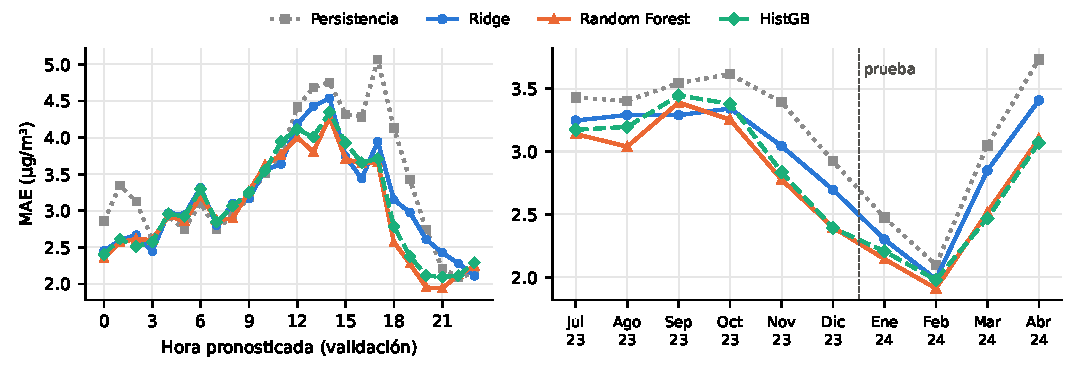
\includegraphics[width=\textwidth]{figures/17_errores_hora_mes.pdf}
\caption{MAE por hora pronosticada en validación (izquierda) y por mes en validación y prueba (derecha). La línea discontinua separa ambos bloques.}
\label{fig:hora-mes}
\end{figure*}

\subsection{Régimen de concentraciones altas}
\label{sec:regimen-alto}
La Fig.~\ref{fig:nivel} agrupa las horas según la concentración observada, usando como cortes la guía diaria de la OMS y sus metas intermedias~\cite{who_aqg_2021}; 50 µg/m³ coincide además con el ECA peruano~\cite{minam_eca_2017}. Esos valores se definen sobre promedios de 24~h y aquí solo sirven para agrupar horas. El MAE crece con la concentración en todos los modelos, y por encima de 50 µg/m³ el sesgo es claramente negativo: los modelos subestiman los episodios. Parte de ese sesgo es mecánica, porque agrupar por el valor observado selecciona las horas en que la concentración subió por encima de lo esperable con la información disponible, y cualquier predictor regresa hacia la media en ellas. Aun así, describe lo que ocurriría en un episodio real.

\begin{figure*}[t]
\centering
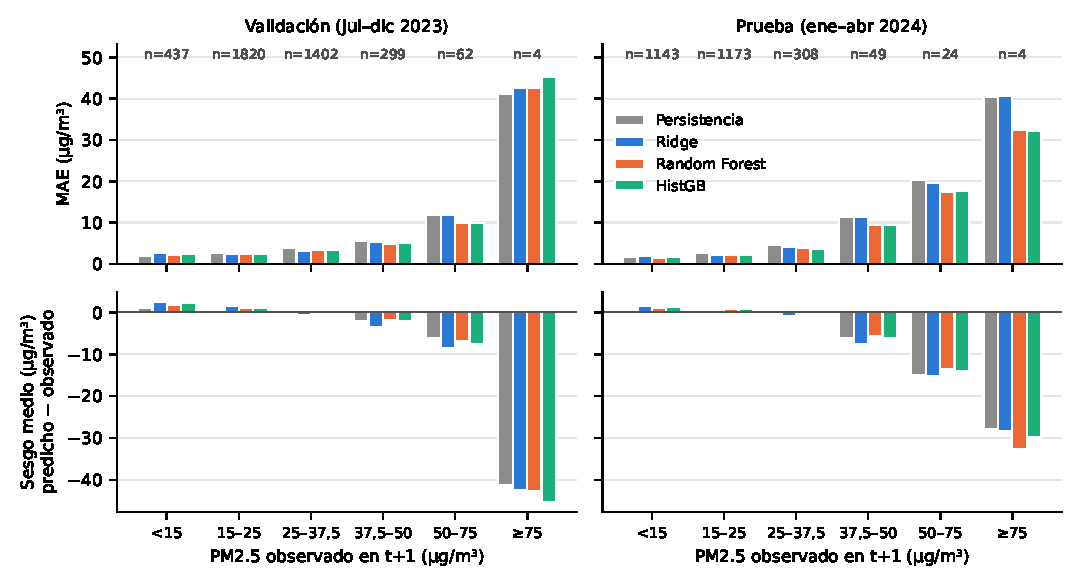
\includegraphics[width=\textwidth]{figures/18_errores_por_nivel.pdf}
\caption{MAE (arriba) y sesgo medio, predicho menos observado (abajo), por nivel de PM2.5 observado en $t+1$. Se indica el número de horas de cada nivel; el último tramo tiene solo cuatro horas por bloque.}
\label{fig:nivel}
\end{figure*}

La Tabla~\ref{tab:regimen} evalúa dos definiciones del régimen alto. La primera es un umbral fijo de 59,25 µg/m³, el percentil 90 de la respuesta en entrenamiento; por el descenso de las concentraciones solo lo superan 16 horas de validación y 17 de prueba. La segunda es el decil superior de cada bloque (desde 36,8 µg/m³ en validación y 27,5 en prueba), con muestra suficiente para comparar. En el decil superior el MAE es entre dos y cuatro veces el del resto de horas (por ejemplo, 5,89 frente a 2,66 para Random Forest en validación y 6,80 frente a 1,92 en prueba). Random Forest y HistGB mejoran a la persistencia en ese decil entre un 8,7~\% y un 18,3~\%, con intervalos que excluyen el cero en ambos bloques, mientras que la mejora de Ridge es pequeña (1,7~\% y 5,3~\%) y en validación no se distingue de cero. Con el umbral fijo, en prueba los árboles reducen el MAE en unos 5,5 µg/m³ frente a la persistencia (IC $[-7{,}8;\,-2{,}5]$ para Random Forest), pero su sesgo sigue cerca de $-22{,}5$ µg/m³; en validación ninguna diferencia es concluyente. Con tan pocas horas, estas cifras son indicativas.

\begin{table}[t]
\centering
\caption{Régimen alto. Umbral fijo: respuesta $\geq 59{,}25$ µg/m³ (p90 de entrenamiento). Decil: 10~\% superior de cada bloque. Mejora frente a persistencia; * indica que el IC 95~\% de la diferencia de MAE excluye el cero.}
\label{tab:regimen}
\small
\setlength{\tabcolsep}{3pt}
\begin{tabular}{@{}lrrrrrr@{}}
\toprule
& \multicolumn{2}{c}{Decil, val.} & \multicolumn{2}{c}{Decil, prueba} & \multicolumn{2}{c}{Umbral, prueba} \\
\cmidrule(lr){2-3}\cmidrule(lr){4-5}\cmidrule(l){6-7}
Modelo & MAE & Mejora & MAE & Mejora & MAE & Mejora \\
\midrule
$n$ & \multicolumn{2}{c}{403} & \multicolumn{2}{c}{272} & \multicolumn{2}{c}{17} \\
Persistencia & 6,74 & -- & 8,08 & -- & 29,05 & -- \\
Ridge & 6,63 & 1,7~\% & 7,65 & 5,3~\%* & 28,28 & 2,6~\% \\
Random Forest & 5,89 & 12,6~\%* & 6,80 & 15,9~\%* & 23,50 & 19,1~\%* \\
HistGB & 6,15 & 8,7~\%* & 6,59 & 18,3~\%* & 23,44 & 19,3~\%* \\
\bottomrule
\end{tabular}
\end{table}

La subestimación persistente es coherente con la limitación señalada en la sección~\ref{sec:no-lineales}: los árboles promedian valores observados en hojas grandes y no pueden anticipar un pico que la historia reciente no anuncia. Sin variables meteorológicas ni de emisiones, el historial de la propia serie no contiene la información necesaria para prever el inicio de un episodio.

\subsection{Respuesta a las preguntas de investigación}
\label{sec:respuestas}
\textbf{P1.} Los modelos de árboles mejoran a la persistencia entre un 9,5~\% y un 11,6~\% en MAE en validación y alrededor de un 14~\% en prueba (unos 0,4 µg/m³ por hora), frente al 7~\% de Ridge. La mejora es estadísticamente consistente, pero pequeña en términos absolutos: la persistencia sigue siendo una referencia exigente a una hora.

\textbf{P2.} El calendario aporta solo en los modelos que pueden combinarlo con el historial. En los de árboles reduce el MAE de validación un 2--3~\%, y el aporte proviene de la hora pronosticada; el día de la semana no aporta en ningún modelo. En los lineales, el calendario empeora ligeramente el MAE.

\textbf{P3.} Sí. En el decil superior el MAE es entre dos y cuatro veces el del resto, y por encima de 50 µg/m³ todos los modelos subestiman de forma sistemática. Los árboles conservan, e incluso amplían, su ventaja relativa sobre la persistencia en ese régimen; la de Ridge se reduce a un 2--5~\% y en validación no se distingue de cero. Ningún modelo resuelve la subestimación de los picos, que es la principal limitación para un uso sanitario del pronóstico.
.
% Requiere booktabs y graphicx. Figuras 15-18: scripts/06_analisis_errores.py.
% Cifras: data/processed/lineales_*.csv, no_lineales_*.csv y errores_*.csv.
\section{Resultados y análisis}
\label{sec:resultados}
Se comparan cuatro modelos sobre las mismas filas: persistencia, Ridge sin calendario (el lineal elegido en la sección~5) y los representantes con calendario de Random Forest y HistGB. Las diferencias de MAE se acompañan de intervalos de confianza del 95~\% obtenidos por bootstrap de bloques móviles de 24 filas consecutivas (2000 réplicas), que conserva la autocorrelación de los errores; los bloques se forman sobre filas, por lo que un hueco de medición puede quedar dentro de un bloque.

\subsection{Comparación global}
\label{sec:comparacion}
La Tabla~\ref{tab:resultados} y la Fig.~\ref{fig:comparacion} resumen el desempeño. En validación, Random Forest obtiene el menor MAE (2,985) y mejora un 11,6~\% sobre la persistencia, frente al 9,5~\% de HistGB y el 7,0~\% de Ridge. En prueba, los dos modelos de árboles quedan prácticamente empatados en MAE (2,413 y 2,428, mejoras de 14,7~\% y 14,2~\%) y HistGB logra el menor RMSE (4,347). Los intervalos de la diferencia con la persistencia excluyen el cero para los tres modelos en ambos bloques. Frente a Ridge, Random Forest reduce el MAE en 0,16 µg/m³ en validación (IC $[-0{,}22;\,-0{,}10]$) y 0,21 en prueba ($[-0{,}28;\,-0{,}15]$); HistGB, en 0,08 ($[-0{,}15;\,-0{,}02]$) y 0,20 ($[-0{,}27;\,-0{,}12]$). La ganancia de los árboles es, por tanto, consistente pero modesta en términos absolutos: del orden de 0,2--0,4 µg/m³ por hora.

\begin{table}[t]
\centering
\caption{Desempeño en validación y prueba. Mejora: reducción porcentual del MAE frente a la persistencia en el mismo bloque. $\Delta$: diferencia de MAE frente a persistencia (µg/m³) con IC 95~\% por bootstrap de bloques.}
\label{tab:resultados}
\small
\setlength{\tabcolsep}{3.5pt}
\begin{tabular}{@{}lrrrrl@{}}
\toprule
Modelo & MAE & RMSE & $R^2$ & Mejora & $\Delta$ [IC 95~\%] \\
\midrule
\multicolumn{6}{@{}l}{\emph{Validación (jul--dic 2023, $n=4024$)}} \\
Persistencia & 3,378 & 5,143 & 0,700 & -- & -- \\
Ridge & 3,141 & 4,755 & 0,744 & 7,0~\% & $-0{,}24$ [$-0{,}29$; $-0{,}18$] \\
Random Forest & \textbf{2,985} & \textbf{4,565} & \textbf{0,764} & 11,6~\% & $-0{,}39$ [$-0{,}47$; $-0{,}32$] \\
HistGB & 3,057 & 4,617 & 0,758 & 9,5~\% & $-0{,}32$ [$-0{,}41$; $-0{,}24$] \\
\midrule
\multicolumn{6}{@{}l}{\emph{Prueba (ene--abr 2024, $n=2701$)}} \\
Persistencia & 2,829 & 5,265 & 0,631 & -- & -- \\
Ridge & 2,626 & 4,766 & 0,698 & 7,2~\% & $-0{,}20$ [$-0{,}27$; $-0{,}13$] \\
Random Forest & \textbf{2,413} & 4,486 & 0,732 & 14,7~\% & $-0{,}42$ [$-0{,}51$; $-0{,}31$] \\
HistGB & 2,428 & \textbf{4,347} & \textbf{0,749} & 14,2~\% & $-0{,}40$ [$-0{,}52$; $-0{,}28$] \\
\bottomrule
\end{tabular}
\end{table}

\begin{figure*}[t]
\centering
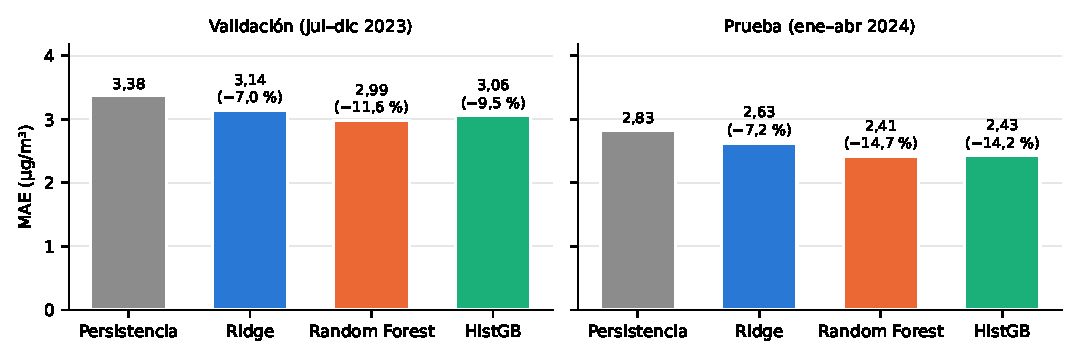
\includegraphics[width=\textwidth]{figures/15_comparacion_modelos.pdf}
\caption{MAE por modelo y bloque. Entre paréntesis, la reducción del MAE frente a la persistencia en el mismo bloque.}
\label{fig:comparacion}
\end{figure*}

El MAE de prueba es menor que el de validación para todos los modelos, incluida la persistencia, y el $R^2$ también es menor. Ambos hechos se explican por el cambio de distribución descrito en la sección~3: enero--abril de 2024 tiene concentraciones más bajas y menos variables, de modo que los errores absolutos se reducen sin que el problema sea más fácil en términos relativos. Por la misma razón, el MAE de la validación cruzada interna (4,82 para Random Forest) es mayor: su primera ventana, en el invierno de 2022, tiene un MAE de 6,68, frente a 3,42 en la tercera.

\subsection{Aporte del calendario}
\label{sec:calendario}
La Tabla~\ref{tab:calendario} compara cada familia con y sin calendario en validación, con la misma búsqueda de hiperparámetros. En los modelos lineales el calendario empeora el MAE alrededor de un 2~\%, con un intervalo que excluye el cero; en los de árboles lo mejora un 3,2~\% (Random Forest) y un 2,4~\% (HistGB), también con intervalos que excluyen el cero. La importancia por permutación (Fig.~\ref{fig:importancia}) localiza el aporte en la hora pronosticada: permutarla aumenta el MAE de validación en 0,36 µg/m³ en Random Forest y 0,49 en HistGB, mientras que permutar el día de la semana no lo cambia. Una interpretación coherente es que el efecto de la hora no es aditivo: las mayores ganancias de los árboles sobre Ridge se concentran entre las 17 y las 21~h (sección~\ref{sec:errores}), cuando la concentración cambia de tendencia a diario, y esa interacción entre hora y nivel reciente no puede representarse con un seno y un coseno sumados linealmente.

\begin{table}[t]
\centering
\caption{MAE de validación sin y con calendario. $\Delta$: con menos sin (µg/m³), IC 95~\% por bootstrap de bloques.}
\label{tab:calendario}
\small
\setlength{\tabcolsep}{3pt}
\begin{tabular}{@{}lrrrl@{}}
\toprule
Familia & Sin & Con & Cambio & $\Delta$ [IC 95~\%] \\
\midrule
Ridge & 3,141 & 3,205 & $+2{,}0$~\% & $0{,}06$ [$0{,}02$; $0{,}11$] \\
Lasso & 3,142 & 3,205 & $+2{,}0$~\% & $0{,}06$ [$0{,}02$; $0{,}11$] \\
Random Forest & 3,083 & 2,985 & $-3{,}2$~\% & $-0{,}10$ [$-0{,}13$; $-0{,}06$] \\
HistGB & 3,132 & 3,057 & $-2{,}4$~\% & $-0{,}07$ [$-0{,}12$; $-0{,}02$] \\
\bottomrule
\end{tabular}
\end{table}

\subsection{Importancia de variables}
\label{sec:importancia}
La importancia se mide como el aumento del MAE de validación al permutar una variable, con 20 repeticiones (Fig.~\ref{fig:importancia}); para la hora y el día se permuta la variable original, de modo que su seno y coseno, o sus indicadores, se alteran juntos. En ambos modelos domina la medición actual: permutarla eleva el MAE en 6,76 (Random Forest) y 6,97 µg/m³ (HistGB). Le siguen la hora (0,36 y 0,49) y el rezago de una hora (0,28 y 0,33); el resto aporta menos de 0,15. Este patrón coincide con la autocorrelación parcial de la sección~3, en la que la dependencia se concentra en los primeros rezagos.

\begin{figure}[t]
\centering
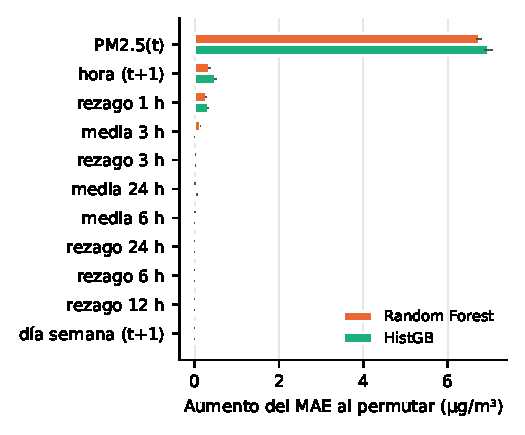
\includegraphics[width=\columnwidth]{figures/16_importancia_variables.pdf}
\caption{Importancia por permutación en validación: aumento del MAE al permutar cada variable (media y desviación de 20 repeticiones).}
\label{fig:importancia}
\end{figure}

Estas cifras tienen tres limitaciones. Primero, las variables de historial están muy correlacionadas: permutar una sola crea combinaciones de entrada que no ocurren en los datos y, a la vez, sus sustitutas pueden compensar su ausencia. Una importancia baja de, por ejemplo, la media de 6~h no implica que la variable sea irrelevante, sino que su información ya está en otras. La distorsión es visible en HistGB, donde permutar conjuntamente las nueve variables de historial aumenta el MAE menos (6,49) que permutar solo la medición actual (6,97). Segundo, la importancia por impureza de Random Forest, calculada en entrenamiento, ordena las variables de forma distinta (medición actual 0,65, media de 3~h 0,21 y rezago de 1~h 0,08) porque reparte el mérito entre variables correlacionadas y favorece las continuas; por eso se reporta solo como contraste. Tercero, ninguna de estas medidas es causal: describen de qué depende el modelo, no qué determina la concentración.

\subsection{Análisis de errores por hora y por mes}
\label{sec:errores}
La Fig.~\ref{fig:hora-mes} desagrega el MAE. Por hora, todos los modelos fallan más entre las 12 y las 15~h de validación, con MAE de 3,7 a 4,8 µg/m³, cuando la concentración sube y cambia con rapidez. La persistencia, que repite el último valor, sufre además en las transiciones: alcanza 5,07 a las 17~h y 3,35 a la 1~h. Allí los árboles obtienen sus mayores ganancias: a las 17~h Random Forest baja a 3,66 frente a 3,95 de Ridge, y a las 19~h, a 2,28 frente a 2,98. En la madrugada y la mañana (3 a 9~h) los cuatro modelos se comportan de forma muy parecida, y entre las 4 y las 7~h la persistencia es incluso ligeramente mejor, lo que indica que en ese tramo la serie cambia poco y la información adicional no aporta.

Por mes, el error es mayor entre septiembre y octubre de 2023 (MAE de 3,2 a 3,6 en todos los modelos) y mínimo en febrero de 2024 (1,9 a 2,1), y vuelve a subir en marzo y abril de 2024. Las diferencias entre meses son mayores que las diferencias entre modelos, por lo que el periodo evaluado condiciona la cifra global tanto como el modelo elegido. El orden de los modelos se mantiene casi todos los meses: la persistencia es la peor en los diez meses, y Random Forest supera a Ridge en nueve, con septiembre de 2023 como excepción.

\begin{figure*}[t]
\centering
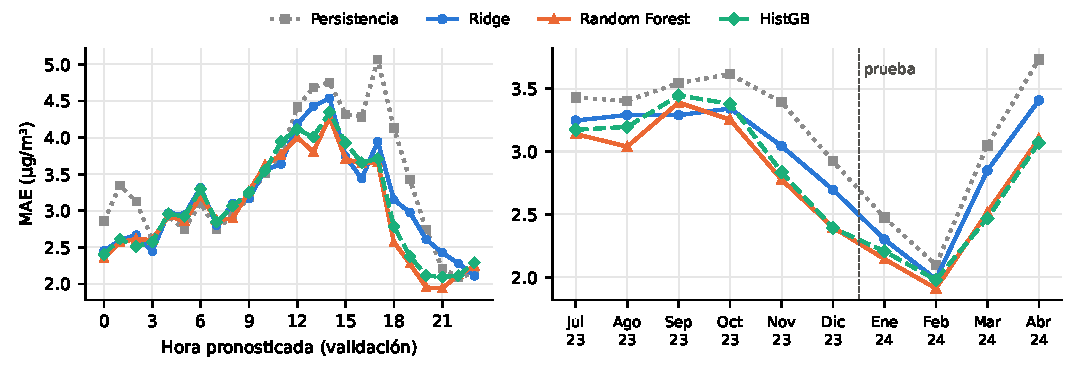
\includegraphics[width=\textwidth]{figures/17_errores_hora_mes.pdf}
\caption{MAE por hora pronosticada en validación (izquierda) y por mes en validación y prueba (derecha). La línea discontinua separa ambos bloques.}
\label{fig:hora-mes}
\end{figure*}

\subsection{Régimen de concentraciones altas}
\label{sec:regimen-alto}
La Fig.~\ref{fig:nivel} agrupa las horas según la concentración observada, usando como cortes la guía diaria de la OMS y sus metas intermedias~\cite{who_aqg_2021}; 50 µg/m³ coincide además con el ECA peruano~\cite{minam_eca_2017}. Esos valores se definen sobre promedios de 24~h y aquí solo sirven para agrupar horas. El MAE crece con la concentración en todos los modelos, y por encima de 50 µg/m³ el sesgo es claramente negativo: los modelos subestiman los episodios. Parte de ese sesgo es mecánica, porque agrupar por el valor observado selecciona las horas en que la concentración subió por encima de lo esperable con la información disponible, y cualquier predictor regresa hacia la media en ellas. Aun así, describe lo que ocurriría en un episodio real.

\begin{figure*}[t]
\centering
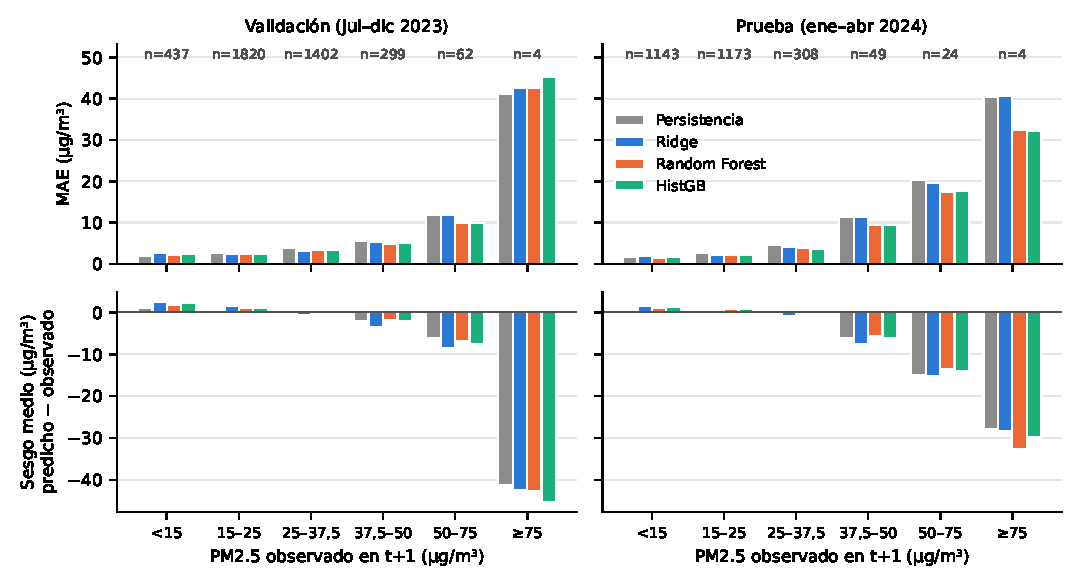
\includegraphics[width=\textwidth]{figures/18_errores_por_nivel.pdf}
\caption{MAE (arriba) y sesgo medio, predicho menos observado (abajo), por nivel de PM2.5 observado en $t+1$. Se indica el número de horas de cada nivel; el último tramo tiene solo cuatro horas por bloque.}
\label{fig:nivel}
\end{figure*}

La Tabla~\ref{tab:regimen} evalúa dos definiciones del régimen alto. La primera es un umbral fijo de 59,25 µg/m³, el percentil 90 de la respuesta en entrenamiento; por el descenso de las concentraciones solo lo superan 16 horas de validación y 17 de prueba. La segunda es el decil superior de cada bloque (desde 36,8 µg/m³ en validación y 27,5 en prueba), con muestra suficiente para comparar. En el decil superior el MAE es entre dos y cuatro veces el del resto de horas (por ejemplo, 5,89 frente a 2,66 para Random Forest en validación y 6,80 frente a 1,92 en prueba). Random Forest y HistGB mejoran a la persistencia en ese decil entre un 8,7~\% y un 18,3~\%, con intervalos que excluyen el cero en ambos bloques, mientras que la mejora de Ridge es pequeña (1,7~\% y 5,3~\%) y en validación no se distingue de cero. Con el umbral fijo, en prueba los árboles reducen el MAE en unos 5,5 µg/m³ frente a la persistencia (IC $[-7{,}8;\,-2{,}5]$ para Random Forest), pero su sesgo sigue cerca de $-22{,}5$ µg/m³; en validación ninguna diferencia es concluyente. Con tan pocas horas, estas cifras son indicativas.

\begin{table}[t]
\centering
\caption{Régimen alto. Umbral fijo: respuesta $\geq 59{,}25$ µg/m³ (p90 de entrenamiento). Decil: 10~\% superior de cada bloque. Mejora frente a persistencia; * indica que el IC 95~\% de la diferencia de MAE excluye el cero.}
\label{tab:regimen}
\small
\setlength{\tabcolsep}{3pt}
\begin{tabular}{@{}lrrrrrr@{}}
\toprule
& \multicolumn{2}{c}{Decil, val.} & \multicolumn{2}{c}{Decil, prueba} & \multicolumn{2}{c}{Umbral, prueba} \\
\cmidrule(lr){2-3}\cmidrule(lr){4-5}\cmidrule(l){6-7}
Modelo & MAE & Mejora & MAE & Mejora & MAE & Mejora \\
\midrule
$n$ & \multicolumn{2}{c}{403} & \multicolumn{2}{c}{272} & \multicolumn{2}{c}{17} \\
Persistencia & 6,74 & -- & 8,08 & -- & 29,05 & -- \\
Ridge & 6,63 & 1,7~\% & 7,65 & 5,3~\%* & 28,28 & 2,6~\% \\
Random Forest & 5,89 & 12,6~\%* & 6,80 & 15,9~\%* & 23,50 & 19,1~\%* \\
HistGB & 6,15 & 8,7~\%* & 6,59 & 18,3~\%* & 23,44 & 19,3~\%* \\
\bottomrule
\end{tabular}
\end{table}

La subestimación persistente es coherente con la limitación señalada en la sección~\ref{sec:no-lineales}: los árboles promedian valores observados en hojas grandes y no pueden anticipar un pico que la historia reciente no anuncia. Sin variables meteorológicas ni de emisiones, el historial de la propia serie no contiene la información necesaria para prever el inicio de un episodio.

\subsection{Respuesta a las preguntas de investigación}
\label{sec:respuestas}
\textbf{P1.} Los modelos de árboles mejoran a la persistencia entre un 9,5~\% y un 11,6~\% en MAE en validación y alrededor de un 14~\% en prueba (unos 0,4 µg/m³ por hora), frente al 7~\% de Ridge. La mejora es estadísticamente consistente, pero pequeña en términos absolutos: la persistencia sigue siendo una referencia exigente a una hora.

\textbf{P2.} El calendario aporta solo en los modelos que pueden combinarlo con el historial. En los de árboles reduce el MAE de validación un 2--3~\%, y el aporte proviene de la hora pronosticada; el día de la semana no aporta en ningún modelo. En los lineales, el calendario empeora ligeramente el MAE.

\textbf{P3.} Sí. En el decil superior el MAE es entre dos y cuatro veces el del resto, y por encima de 50 µg/m³ todos los modelos subestiman de forma sistemática. Los árboles conservan, e incluso amplían, su ventaja relativa sobre la persistencia en ese régimen; la de Ridge se reduce a un 2--5~\% y en validación no se distingue de cero. Ningún modelo resuelve la subestimación de los picos, que es la principal limitación para un uso sanitario del pronóstico.
.
% Requiere booktabs y graphicx. Figuras 15-18: scripts/06_analisis_errores.py.
% Cifras: data/processed/lineales_*.csv, no_lineales_*.csv y errores_*.csv.
\section{Resultados y análisis}
\label{sec:resultados}
Se comparan cuatro modelos sobre las mismas filas: persistencia, Ridge sin calendario (el lineal elegido en la sección~5) y los representantes con calendario de Random Forest y HistGB. Las diferencias de MAE se acompañan de intervalos de confianza del 95~\% obtenidos por bootstrap de bloques móviles de 24 filas consecutivas (2000 réplicas), que conserva la autocorrelación de los errores; los bloques se forman sobre filas, por lo que un hueco de medición puede quedar dentro de un bloque.

\subsection{Comparación global}
\label{sec:comparacion}
La Tabla~\ref{tab:resultados} y la Fig.~\ref{fig:comparacion} resumen el desempeño. En validación, Random Forest obtiene el menor MAE (2,985) y mejora un 11,6~\% sobre la persistencia, frente al 9,5~\% de HistGB y el 7,0~\% de Ridge. En prueba, los dos modelos de árboles quedan prácticamente empatados en MAE (2,413 y 2,428, mejoras de 14,7~\% y 14,2~\%) y HistGB logra el menor RMSE (4,347). Los intervalos de la diferencia con la persistencia excluyen el cero para los tres modelos en ambos bloques. Frente a Ridge, Random Forest reduce el MAE en 0,16 µg/m³ en validación (IC $[-0{,}22;\,-0{,}10]$) y 0,21 en prueba ($[-0{,}28;\,-0{,}15]$); HistGB, en 0,08 ($[-0{,}15;\,-0{,}02]$) y 0,20 ($[-0{,}27;\,-0{,}12]$). La ganancia de los árboles es, por tanto, consistente pero modesta en términos absolutos: del orden de 0,2--0,4 µg/m³ por hora.

\begin{table}[t]
\centering
\caption{Desempeño en validación y prueba. Mejora: reducción porcentual del MAE frente a la persistencia en el mismo bloque. $\Delta$: diferencia de MAE frente a persistencia (µg/m³) con IC 95~\% por bootstrap de bloques.}
\label{tab:resultados}
\small
\setlength{\tabcolsep}{3.5pt}
\begin{tabular}{@{}lrrrrl@{}}
\toprule
Modelo & MAE & RMSE & $R^2$ & Mejora & $\Delta$ [IC 95~\%] \\
\midrule
\multicolumn{6}{@{}l}{\emph{Validación (jul--dic 2023, $n=4024$)}} \\
Persistencia & 3,378 & 5,143 & 0,700 & -- & -- \\
Ridge & 3,141 & 4,755 & 0,744 & 7,0~\% & $-0{,}24$ [$-0{,}29$; $-0{,}18$] \\
Random Forest & \textbf{2,985} & \textbf{4,565} & \textbf{0,764} & 11,6~\% & $-0{,}39$ [$-0{,}47$; $-0{,}32$] \\
HistGB & 3,057 & 4,617 & 0,758 & 9,5~\% & $-0{,}32$ [$-0{,}41$; $-0{,}24$] \\
\midrule
\multicolumn{6}{@{}l}{\emph{Prueba (ene--abr 2024, $n=2701$)}} \\
Persistencia & 2,829 & 5,265 & 0,631 & -- & -- \\
Ridge & 2,626 & 4,766 & 0,698 & 7,2~\% & $-0{,}20$ [$-0{,}27$; $-0{,}13$] \\
Random Forest & \textbf{2,413} & 4,486 & 0,732 & 14,7~\% & $-0{,}42$ [$-0{,}51$; $-0{,}31$] \\
HistGB & 2,428 & \textbf{4,347} & \textbf{0,749} & 14,2~\% & $-0{,}40$ [$-0{,}52$; $-0{,}28$] \\
\bottomrule
\end{tabular}
\end{table}

\begin{figure*}[t]
\centering
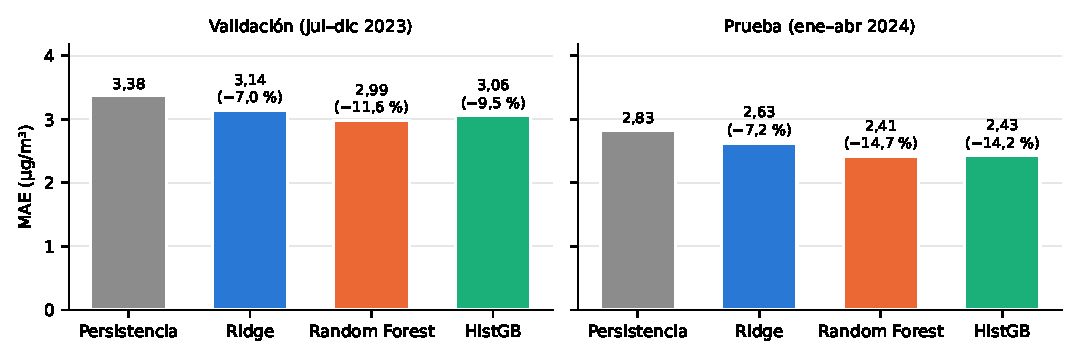
\includegraphics[width=\textwidth]{figures/15_comparacion_modelos.pdf}
\caption{MAE por modelo y bloque. Entre paréntesis, la reducción del MAE frente a la persistencia en el mismo bloque.}
\label{fig:comparacion}
\end{figure*}

El MAE de prueba es menor que el de validación para todos los modelos, incluida la persistencia, y el $R^2$ también es menor. Ambos hechos se explican por el cambio de distribución descrito en la sección~3: enero--abril de 2024 tiene concentraciones más bajas y menos variables, de modo que los errores absolutos se reducen sin que el problema sea más fácil en términos relativos. Por la misma razón, el MAE de la validación cruzada interna (4,82 para Random Forest) es mayor: su primera ventana, en el invierno de 2022, tiene un MAE de 6,68, frente a 3,42 en la tercera.

\subsection{Aporte del calendario}
\label{sec:calendario}
La Tabla~\ref{tab:calendario} compara cada familia con y sin calendario en validación, con la misma búsqueda de hiperparámetros. En los modelos lineales el calendario empeora el MAE alrededor de un 2~\%, con un intervalo que excluye el cero; en los de árboles lo mejora un 3,2~\% (Random Forest) y un 2,4~\% (HistGB), también con intervalos que excluyen el cero. La importancia por permutación (Fig.~\ref{fig:importancia}) localiza el aporte en la hora pronosticada: permutarla aumenta el MAE de validación en 0,36 µg/m³ en Random Forest y 0,49 en HistGB, mientras que permutar el día de la semana no lo cambia. Una interpretación coherente es que el efecto de la hora no es aditivo: las mayores ganancias de los árboles sobre Ridge se concentran entre las 17 y las 21~h (sección~\ref{sec:errores}), cuando la concentración cambia de tendencia a diario, y esa interacción entre hora y nivel reciente no puede representarse con un seno y un coseno sumados linealmente.

\begin{table}[t]
\centering
\caption{MAE de validación sin y con calendario. $\Delta$: con menos sin (µg/m³), IC 95~\% por bootstrap de bloques.}
\label{tab:calendario}
\small
\setlength{\tabcolsep}{3pt}
\begin{tabular}{@{}lrrrl@{}}
\toprule
Familia & Sin & Con & Cambio & $\Delta$ [IC 95~\%] \\
\midrule
Ridge & 3,141 & 3,205 & $+2{,}0$~\% & $0{,}06$ [$0{,}02$; $0{,}11$] \\
Lasso & 3,142 & 3,205 & $+2{,}0$~\% & $0{,}06$ [$0{,}02$; $0{,}11$] \\
Random Forest & 3,083 & 2,985 & $-3{,}2$~\% & $-0{,}10$ [$-0{,}13$; $-0{,}06$] \\
HistGB & 3,132 & 3,057 & $-2{,}4$~\% & $-0{,}07$ [$-0{,}12$; $-0{,}02$] \\
\bottomrule
\end{tabular}
\end{table}

\subsection{Importancia de variables}
\label{sec:importancia}
La importancia se mide como el aumento del MAE de validación al permutar una variable, con 20 repeticiones (Fig.~\ref{fig:importancia}); para la hora y el día se permuta la variable original, de modo que su seno y coseno, o sus indicadores, se alteran juntos. En ambos modelos domina la medición actual: permutarla eleva el MAE en 6,76 (Random Forest) y 6,97 µg/m³ (HistGB). Le siguen la hora (0,36 y 0,49) y el rezago de una hora (0,28 y 0,33); el resto aporta menos de 0,15. Este patrón coincide con la autocorrelación parcial de la sección~3, en la que la dependencia se concentra en los primeros rezagos.

\begin{figure}[t]
\centering
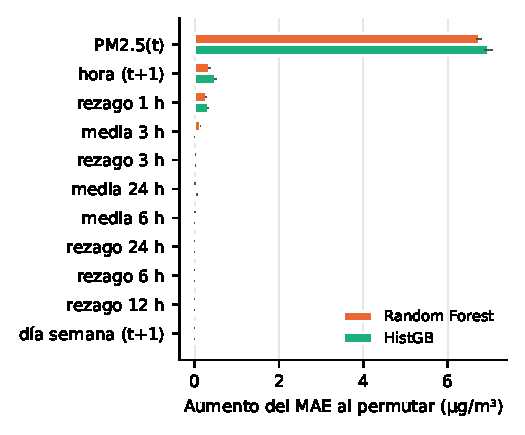
\includegraphics[width=\columnwidth]{figures/16_importancia_variables.pdf}
\caption{Importancia por permutación en validación: aumento del MAE al permutar cada variable (media y desviación de 20 repeticiones).}
\label{fig:importancia}
\end{figure}

Estas cifras tienen tres limitaciones. Primero, las variables de historial están muy correlacionadas: permutar una sola crea combinaciones de entrada que no ocurren en los datos y, a la vez, sus sustitutas pueden compensar su ausencia. Una importancia baja de, por ejemplo, la media de 6~h no implica que la variable sea irrelevante, sino que su información ya está en otras. La distorsión es visible en HistGB, donde permutar conjuntamente las nueve variables de historial aumenta el MAE menos (6,49) que permutar solo la medición actual (6,97). Segundo, la importancia por impureza de Random Forest, calculada en entrenamiento, ordena las variables de forma distinta (medición actual 0,65, media de 3~h 0,21 y rezago de 1~h 0,08) porque reparte el mérito entre variables correlacionadas y favorece las continuas; por eso se reporta solo como contraste. Tercero, ninguna de estas medidas es causal: describen de qué depende el modelo, no qué determina la concentración.

\subsection{Análisis de errores por hora y por mes}
\label{sec:errores}
La Fig.~\ref{fig:hora-mes} desagrega el MAE. Por hora, todos los modelos fallan más entre las 12 y las 15~h de validación, con MAE de 3,7 a 4,8 µg/m³, cuando la concentración sube y cambia con rapidez. La persistencia, que repite el último valor, sufre además en las transiciones: alcanza 5,07 a las 17~h y 3,35 a la 1~h. Allí los árboles obtienen sus mayores ganancias: a las 17~h Random Forest baja a 3,66 frente a 3,95 de Ridge, y a las 19~h, a 2,28 frente a 2,98. En la madrugada y la mañana (3 a 9~h) los cuatro modelos se comportan de forma muy parecida, y entre las 4 y las 7~h la persistencia es incluso ligeramente mejor, lo que indica que en ese tramo la serie cambia poco y la información adicional no aporta.

Por mes, el error es mayor entre septiembre y octubre de 2023 (MAE de 3,2 a 3,6 en todos los modelos) y mínimo en febrero de 2024 (1,9 a 2,1), y vuelve a subir en marzo y abril de 2024. Las diferencias entre meses son mayores que las diferencias entre modelos, por lo que el periodo evaluado condiciona la cifra global tanto como el modelo elegido. El orden de los modelos se mantiene casi todos los meses: la persistencia es la peor en los diez meses, y Random Forest supera a Ridge en nueve, con septiembre de 2023 como excepción.

\begin{figure*}[t]
\centering
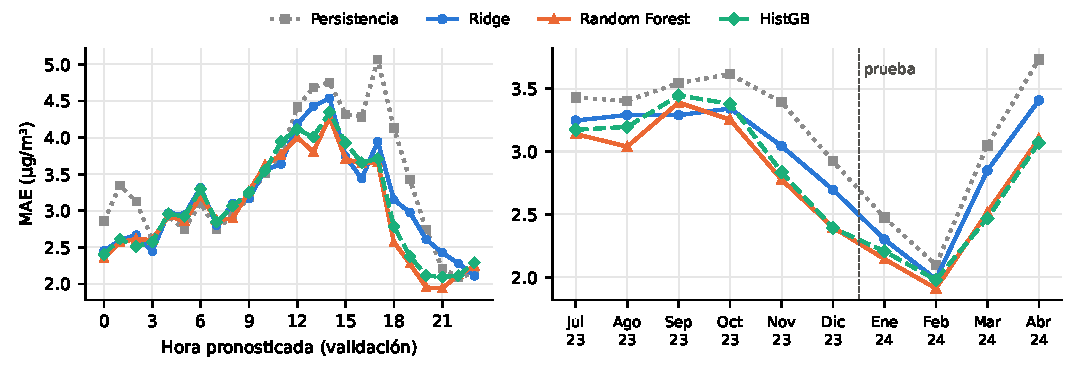
\includegraphics[width=\textwidth]{figures/17_errores_hora_mes.pdf}
\caption{MAE por hora pronosticada en validación (izquierda) y por mes en validación y prueba (derecha). La línea discontinua separa ambos bloques.}
\label{fig:hora-mes}
\end{figure*}

\subsection{Régimen de concentraciones altas}
\label{sec:regimen-alto}
La Fig.~\ref{fig:nivel} agrupa las horas según la concentración observada, usando como cortes la guía diaria de la OMS y sus metas intermedias~\cite{who_aqg_2021}; 50 µg/m³ coincide además con el ECA peruano~\cite{minam_eca_2017}. Esos valores se definen sobre promedios de 24~h y aquí solo sirven para agrupar horas. El MAE crece con la concentración en todos los modelos, y por encima de 50 µg/m³ el sesgo es claramente negativo: los modelos subestiman los episodios. Parte de ese sesgo es mecánica, porque agrupar por el valor observado selecciona las horas en que la concentración subió por encima de lo esperable con la información disponible, y cualquier predictor regresa hacia la media en ellas. Aun así, describe lo que ocurriría en un episodio real.

\begin{figure*}[t]
\centering
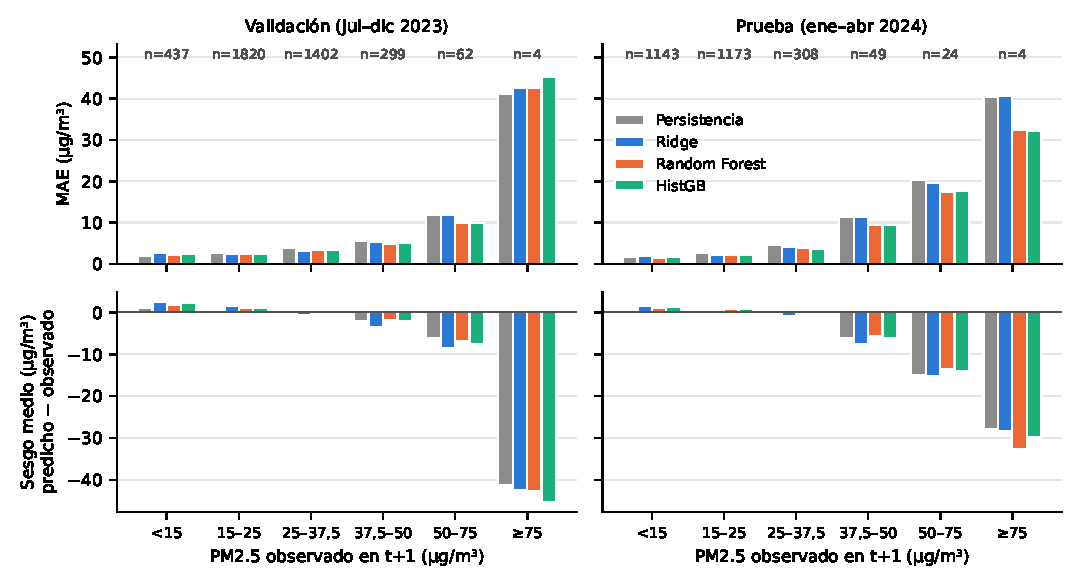
\includegraphics[width=\textwidth]{figures/18_errores_por_nivel.pdf}
\caption{MAE (arriba) y sesgo medio, predicho menos observado (abajo), por nivel de PM2.5 observado en $t+1$. Se indica el número de horas de cada nivel; el último tramo tiene solo cuatro horas por bloque.}
\label{fig:nivel}
\end{figure*}

La Tabla~\ref{tab:regimen} evalúa dos definiciones del régimen alto. La primera es un umbral fijo de 59,25 µg/m³, el percentil 90 de la respuesta en entrenamiento; por el descenso de las concentraciones solo lo superan 16 horas de validación y 17 de prueba. La segunda es el decil superior de cada bloque (desde 36,8 µg/m³ en validación y 27,5 en prueba), con muestra suficiente para comparar. En el decil superior el MAE es entre dos y cuatro veces el del resto de horas (por ejemplo, 5,89 frente a 2,66 para Random Forest en validación y 6,80 frente a 1,92 en prueba). Random Forest y HistGB mejoran a la persistencia en ese decil entre un 8,7~\% y un 18,3~\%, con intervalos que excluyen el cero en ambos bloques, mientras que la mejora de Ridge es pequeña (1,7~\% y 5,3~\%) y en validación no se distingue de cero. Con el umbral fijo, en prueba los árboles reducen el MAE en unos 5,5 µg/m³ frente a la persistencia (IC $[-7{,}8;\,-2{,}5]$ para Random Forest), pero su sesgo sigue cerca de $-22{,}5$ µg/m³; en validación ninguna diferencia es concluyente. Con tan pocas horas, estas cifras son indicativas.

\begin{table}[t]
\centering
\caption{Régimen alto. Umbral fijo: respuesta $\geq 59{,}25$ µg/m³ (p90 de entrenamiento). Decil: 10~\% superior de cada bloque. Mejora frente a persistencia; * indica que el IC 95~\% de la diferencia de MAE excluye el cero.}
\label{tab:regimen}
\small
\setlength{\tabcolsep}{3pt}
\begin{tabular}{@{}lrrrrrr@{}}
\toprule
& \multicolumn{2}{c}{Decil, val.} & \multicolumn{2}{c}{Decil, prueba} & \multicolumn{2}{c}{Umbral, prueba} \\
\cmidrule(lr){2-3}\cmidrule(lr){4-5}\cmidrule(l){6-7}
Modelo & MAE & Mejora & MAE & Mejora & MAE & Mejora \\
\midrule
$n$ & \multicolumn{2}{c}{403} & \multicolumn{2}{c}{272} & \multicolumn{2}{c}{17} \\
Persistencia & 6,74 & -- & 8,08 & -- & 29,05 & -- \\
Ridge & 6,63 & 1,7~\% & 7,65 & 5,3~\%* & 28,28 & 2,6~\% \\
Random Forest & 5,89 & 12,6~\%* & 6,80 & 15,9~\%* & 23,50 & 19,1~\%* \\
HistGB & 6,15 & 8,7~\%* & 6,59 & 18,3~\%* & 23,44 & 19,3~\%* \\
\bottomrule
\end{tabular}
\end{table}

La subestimación persistente es coherente con la limitación señalada en la sección~\ref{sec:no-lineales}: los árboles promedian valores observados en hojas grandes y no pueden anticipar un pico que la historia reciente no anuncia. Sin variables meteorológicas ni de emisiones, el historial de la propia serie no contiene la información necesaria para prever el inicio de un episodio.

\subsection{Respuesta a las preguntas de investigación}
\label{sec:respuestas}
\textbf{P1.} Los modelos de árboles mejoran a la persistencia entre un 9,5~\% y un 11,6~\% en MAE en validación y alrededor de un 14~\% en prueba (unos 0,4 µg/m³ por hora), frente al 7~\% de Ridge. La mejora es estadísticamente consistente, pero pequeña en términos absolutos: la persistencia sigue siendo una referencia exigente a una hora.

\textbf{P2.} El calendario aporta solo en los modelos que pueden combinarlo con el historial. En los de árboles reduce el MAE de validación un 2--3~\%, y el aporte proviene de la hora pronosticada; el día de la semana no aporta en ningún modelo. En los lineales, el calendario empeora ligeramente el MAE.

\textbf{P3.} Sí. En el decil superior el MAE es entre dos y cuatro veces el del resto, y por encima de 50 µg/m³ todos los modelos subestiman de forma sistemática. Los árboles conservan, e incluso amplían, su ventaja relativa sobre la persistencia en ese régimen; la de Ridge se reduce a un 2--5~\% y en validación no se distingue de cero. Ningún modelo resuelve la subestimación de los picos, que es la principal limitación para un uso sanitario del pronóstico.
